\documentclass{article}
\usepackage[utf8]{inputenc}
\usepackage{adjustbox}
\usepackage{graphicx}
\usepackage{amsmath,amssymb,latexsym}
\usepackage{fullpage}
\usepackage{enumitem}
\usepackage{hyperref}
\usepackage{url}
\usepackage{cite}

\hypersetup{
    colorlinks=true,
    linkcolor=blue,
    filecolor=magenta,      
    urlcolor=cyan,
}

\setlength{\parindent}{0 pt}
\setlength{\parskip  }{5.5 pt}

\renewcommand{\labelitemii}{$\circ$}

\title{Research Proposal:\\Revisiting Grocery Recognition using TensorFlow}
\author{Dilip Thiagarajan, Samuel C.\ Hoffman}
\date{June 20, 2016}


\begin{document}

\maketitle

\section{Introduction}

As the need for assistive technology for the visually impaired becomes more prominent and feasible with the use of machine learning, we revisit the problem of using pictures of objects taken in ideal conditions to recognize more common scenes of these same objects. This problem encompasses several possible applications, but in this study, we will specifically look at grocery products sold in Mattin's, a local café on the Cornell campus in Ithaca. In essence, we will revisit the study conducted by Merler, Galleguillos, and Belongie \cite{merler07} but with a more modern approach involving the tools contained in TensorFlow \cite{tensorflow15}.
\\ \\
The main problem we hope to address by conducting this study is paramount to maintaining the state of assistive technology: ideally, training data and testing data would be obtained from the same distribution of data. However, in real-world application, it is more convenient to obtain training data from more well-kept databases, such as the web or dedicated databases. As a result, using the tools offered in TensorFlow, we intend to design a portable system that can recognize the groceries in Mattin's, trained on images taken from both an ideal and realistic environment.
\\ \\
Specifically, the purpose of this study will be to build a database of images encompassing the inventory of Mattin's ranging from ideal to realistic shots, as well as to use various approaches to actually recognize the grocery products in Mattin's. This will include color histogram matching, SIFT matching, compared with training a neural network that takes image pairs as input (where the image pair consists of an ideal and realistic shot of a grocery object in Mattin's) for classification.
\\ \\
Our ultimate goal in beginning this study is to achieve real-time recognition and localization from a camera. 

\section{Data and Methodology}

To begin, we will need to obtain the relevant types of data for input. As mentioned in the previous study, one database that can be used is the \href{http://grozi.calit2.net/grozi.html}{GroZi-120 database}, which is a database of 120 products with images of objects, ranging over various attributes of the image, and where each product has two different representations: either \textit{in situ}, i.e. in a realistic environment, or \textit{in vitro}, i.e. in an idealistic environment. Another possible way to scrape data could be to use Google searches, and take a sample of the top image hits as training/test data.
\\ \\
Additionally, data would be obtained from Mattin's in person, and due to the changing inventory, images and videos can be taken periodically of each product in the whole inventory to better recognize the inventory, given the varying nature of the products sold. To better train the network being used, photos and videos taken in person will vary in scale and lighting to simulate a more realistic environment.
\\ \\
Once the relevant data has been obtained, it will be used independently on each localization and recognition algorithm, as well as arranged into pairwise input to be used for training on a convolutional neural network built in TensorFlow. Specifically, we will build a sample of several neural networks built in TensorFlow (which will be chosen from the set of all possible networks by using distinctive heuristics) and see how they perform compared to each other on various samplings of training and testing data. Once we have selected the network that performs best, we will compare the results of the standard algorithms with the new accumulation of data to the results in the previous study, as well as comparing how the chosen network built in TensorFlow performs compared to other algorithms on the new accumulation of data.

\section{Related Works}

Given that the scope of computer vision has drastically changed over the past decade with the introduction of deep learning with neural networks, a lot of work has been done towards building tools and studying specific applications. With the ultimate goal of generalized, fine-grained image classification in mind, these tools and studies would prove useful in our own study.

\subsection{Relevant Computer Vision Tools}

As mentioned, deep learning has revolutionized the landscape of computer vision. Nonetheless, there were some frameworks which allowed for image classification, including things like OpenCV in Python, VLFeat, VLX libraries written in C++, and tools like WEKA, but with the advent of deep learning in the past few years, and with the progress they've made on well-known datasets, such as MNIST, CIFAR-10, and ImageNet, we will proceed with using these deep learning frameworks as opposed to the libraries that preceded them.
\\ \\
Several deep learning frameworks have been introduced in the past few years, including libraries such as Theano, Torch, Caffe, and TensorFlow. Our choice of using TensorFlow is somewhat arbitrary, although given it's recency, it does offer several advantages over the other frameworks. Lipton brings up several of these points in his analysis of TensorFlow against other deep learning frameworks.
\\ \\
While TensorFlow is not fundamentally different from Theano or Torch, and Caffe was essentially developed specifically for implementing convolutional neural networks, which is what will be used throughout this study, TensorFlow allows the user to write in Python, which is arguably much simpler to handle than Lua, C++, or Cuda. While Caffe also has Python bindings for running models, it's very inconvenient to define new models or different kinds of layers without adding a large portion of C++ code to their codebase \cite{lipton15}.
\\ \\
In addition, because Python is the main language of use, TensorFlow allows for integration with any other workflow necessary in the grand scheme of the study, whether it be a web server to demonstrate the application, or the use of some open-source scientific computing tool (especially libraries like NumPy and Scikit-learn) \cite{lipton15}. Moreover, TensorFlow works seamlessly when running with multiple GPUs, and the code compiles in very little time. 

\subsection{Relevant Studies}

Our work will build heavily on the study by Merler et al.\ (2007). Other attempts to improve upon the results of the GroZi baseline include a paper by George et al.\ (2015) who used a text-based approach for recognizing classes \cite{george15}. We believe we can further improve upon this with a full deep learning architecture.
\\ \\
The use of deep convolutional neural networks (ConvNets) has revolutionized the field of object recognition and state-of-the-art networks have even surpassed human-level performance in some areas \cite{he15,russakovsky14}. We hope to leverage these breakthroughs to create a network which can discriminate between specific products (in this case, those sold at Mattin's). However, competitions such as the ImageNet Large Scale Visual Recognition Challenge (ILSVRC), which have pushed the limits of ConvNets, are usually focused on general recognition of more coarse-grained categories whereas our goal is much more fine-grained so we must find a way to adapt these broad classifiers to our needs.
\\ \\
One approach is to train a manageably-sized network from scratch on our data set. This allows us to learn deep features important to our classes while still being able to iterate quickly. Since the trend of the past couple years has tended toward larger and more complex networks which may take days to train, we could choose a slightly older but still powerful model such as AlexNet, the ILSVRC winner from 2012 \cite{krizhevsky12}.
\\ \\
Another approach is to fine-tune a state-of-the-art network by replacing the last layer and retraining with our data, starting with the fully-trained weights for the other layers. The early layers in most ConvNets have general functions such as blob detection which are useful for many different applications. If we start out with a network which can identify many higher-order features and then train it to learn class-specific features, we can achieve a very powerful model without spending so long training from scratch \cite{donahue13}. The drawback is that we may need to fine-tune multiple layers to get the best results which, for a state-of-the-art network, may still be a slow process.
\\ \\
We will be benchmarking both approaches and comparing them to the previous baselines mentioned above.
\\ \\
Another important aspect of this project is localization of detected objects in the video frame. Again, there have been great strides recently in this area toward real-time detection with localization particularly using Region Proposal Networks (RPNs). State-of-the-art systems have achieved near-real-time speeds of 5~fps with very deep networks which is fast enough for our purposes \cite{ren15}.

\section{Milestones}

Completed:

\begin{itemize}

	\item Train basic network on a single class (Tide laundry detergent)

	\item Output basic performance characteristics (ROC curve, precision/recall)

\end{itemize}

To do:

\begin{itemize}

	\item Train manageably-sized network (such as AlexNet) from scratch on a single class
	\begin{itemize}
		\item \textit{Dilip: June 20--June 27}
	\end{itemize}

	\item Fine-tune a large network for a single class
	\begin{itemize}
		\item \textit{Sam: June 20--June 27}
	\end{itemize}

	\item Produce framework for outputting performance characteristics for any underlying architecture
	\begin{itemize}
		\item \textit{Both: June 24--July 1}
	\end{itemize}

	\item Generalize both approaches above to all 120 categories in GroZi-120
	\begin{itemize}
		\item \textit{Both: June 24--July 4}
	\end{itemize}

	\item Incorporate a Region Proposal Network for localization of objects in a single, full video frame
	\begin{itemize}
		\item \textit{Both: July 4--July 13}
	\end{itemize}

	\item Create a framework for applying the full workflow on recorded video of store shelves from the GroZi dataset
	\begin{itemize}
		\item \textit{Both: July 13--July 25}
	\end{itemize}

	\item Record shelf footage in Mattin's Café and test system
	\begin{itemize}
		\item \textit{Both: Late July/Early August}
	\end{itemize}

	\item Incorporate framework into an application using real-time camera data
	\begin{itemize}
		\item \textit{Both: July 25--August 12}
	\end{itemize}

	\item Make improvements to recognition network architecture for speed or accuracy as necessary
	\begin{itemize}
		\item \textit{Both: August 1--August 12}
	\end{itemize}

	\item Produce a continuity report for reference in future work
	\begin{itemize}
		\item \textit{Both: July 4--August 19}
	\end{itemize}

\end{itemize}

\begin{figure}[h]
	\caption{Gantt chart depicting the tentative timeline}
	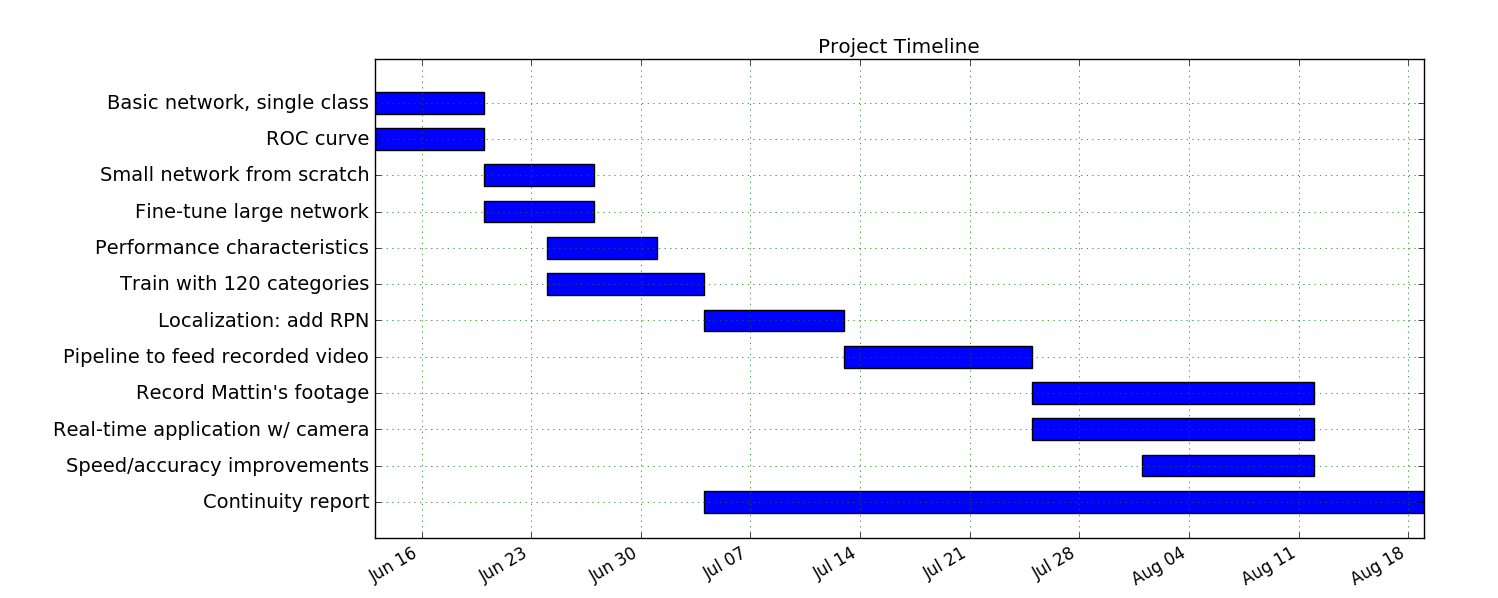
\includegraphics[width=\textwidth]{gantt.png}
\end{figure}

\newpage
\bibliographystyle{abbrv}
\bibliography{Proposal}

\end{document}